\section{\glsentrylong{mpbsm}}

\subsection{\label{subsec:smgeneral}\glsentrytext{sm} in General}
Szeliski defines \gls{sm} \cite[p. 469]{Szeliski2011} as ``the process of taking two or more images and estimating a 3D model of the scene by finding matching pixels in the images and converting their 2D positions into 3D depths.''  It is essentially an attempt to replicate one of the techniques the brain uses to provide depth perception,\footnote{The brain has others, such as exploiting familiarity with everyday objects to estimate their actual size, and thus their rough distance from the eyes.} namely correlating the images received from each eye to estimate the distances to objects within view, but using digital images and a computer.

Indeed, \gls{sm} is not the only method for computer depth perception in use \cite{Sinha2020}.  Other approaches include, for example, Structured Light \cite{Giancola2018}, Time-of-Flight \cite{Hansard2013} and LiDAR \cite{Dong2017}.  \Gls{sm} has some advantages over those other techniques, though.  It is the only one which is entirely passive, \ie{} it takes in data from the environment without interacting with it in some way, whereas the other three all involve projecting some form of light into the environment.  It is also arguably quicker to perform the necessary observations of the environment than the other methods, in that only a single pair of images need be captured, which can be accomplished in the time it takes for the pixel values to be read from the sensor planes into storage.  The choice of which method is most appropriate depends heavily upon the intended use of the computerised depth perception.  Or, if sufficient processing power is available, two or more of them can be used in combination to offset each other's weaknesses \cite{Zanuttigh2016}.

The `canonical' stereo camera arrangement is two cameras arranged in parallel, with a small horizontal offset between them.  This configuration leads to a general expectation that changes in the points in the scene will be shifted along one image's x-axis as compared to the other image's.  The identified distance of a shift is the \gls{disparity}, and is used with other information about the cameras to compute an estimate to the matched points in the scene.  Generally, it is \fxnote*{name of assumption?}{assumed} that points in the image from the left camera will appear further to the right in said image as compared the same point in the right camera's image, and vice versa.

\begin{figure}
    \centering
    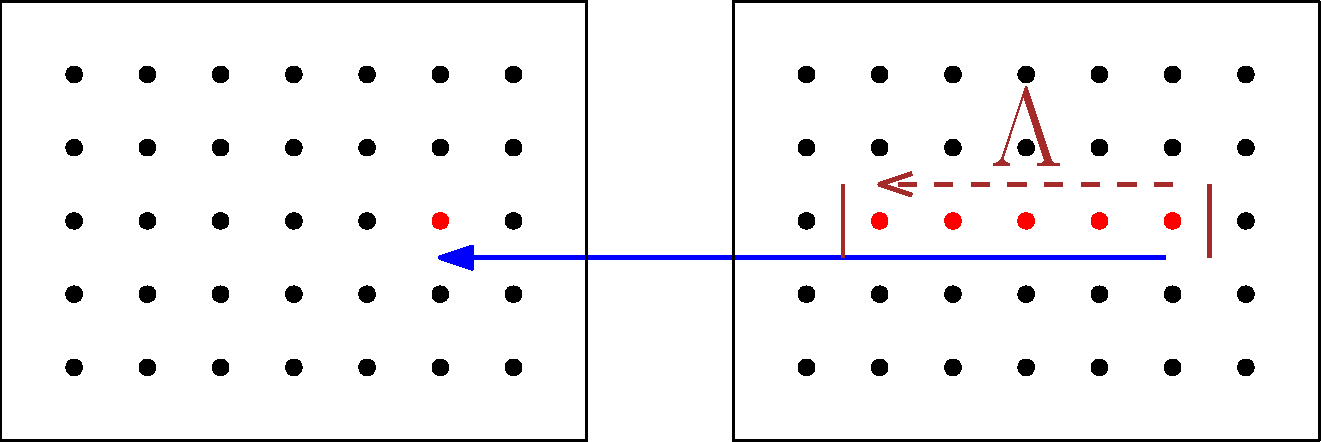
\includegraphics[width=1.0\textwidth]{chapters/litreview/images/stereo_matching-eps-converted-to.pdf}
    \caption[Diagram of the basic process of \gls{sm}]{Diagram of the basic process of \gls{sm}. In this instance, for each pixel in the left image, a horizontal range of the pixels in the right image are searched, to find the one on the right that matches most closely to the one on the left. This has the effect that the \gls{disparitymap} is from the perspective of the left camera. The red dots represent the compared pixels. The brown dashed arrow and vertical bars represent the range of pixels in the right image to compute matching scores against. The length of the range is the lesser of the number of pixels before reaching the left border of the image, or the maximum \gls{disparity}, which is a parameter set by the user and represented here by \(\Lambda\).  Image from \cite{bsmpcvpic}.}
    \label{fig:stereomatchingbasic}
\end{figure}

In the general case \gls{sm} is impossible to perform perfectly because it is an ill-posed problem \cite{Gimelfarb1998}.  Going from a three-dimensional scene to a two-dimensional image necessarily involves a loss of information.  For any given image there are potentially an unbounded number of possible real-world scenes that could produce said image.  Using multiple images -- the more the better -- for \gls{sm} permits some recovery of information, but the process inevitably suffers from various sources of noise (where `noise' is defined broadly).

Liu \textit{et al.} \cite{Liu2005} describe four types of noise:  Signal, geometric, electronic and optical.  Signal noise arises from the normal operation of digital cameras, and electronic from differences between the internal operation of cameras used to capture images from different perspectives of the same scene.  Optical noise mainly stems from differences in the intensity and colour of light seen by the cameras at different perspectives when capturing images of the scene, caused by differences in the interactions between the objects of the scene and the available light sources at different points.  Lastly, geometric noise is a natural consequence of the fact that different perspectives must be used, and can be caused by issues as simple as the fact that points visible in one scene may not be visible in the other -- so-called `occlusions', caused by one part of the scene obscuring another part.

A key consequence of the last source of noise is the fact that, even in ideal circumstances with multiple `perfect' cameras, flawless lighting throughout the scene and \fxnote*{Provide reference for Lambertian surfaces}{objects which do not reflect light differently at different parts of their surfaces}, occlusions mean that for an arbitrary scene it is impossible to be certain a given algorithm has achieved a perfect reconstruction of the depths of the scene \cite{Gimelfarb1998}.  Strictly speaking, it \emph{is} possible that \gls{sm} produces an entirely accurate \gls{disparitymap}, but there would be no way to know without the use of additional information.

\fxwarning[inline,nomargin]{Include some example images to show the idea of stereo matching?}

\subsubsection{Image Rectification}
To reduce the computational complexity involved in performing \gls{sm}, many, perhaps most, algorithms only directly compare pixels along a single line in each image, typically the same horizontal line \cite[Ch. 11]{Szeliski2011}.  If the lines in the two images do not correspond to roughly the same part of the scene, then the matching process will likely fare poorly.  Such a discordance can occur when the cameras were not adequately aligned in terms of their spatial positions and angles relative to each other at the time of mutual image capture.

To overcome the challenges caused by mismatched lines, stereo image pairs are usually `rectified' (see \eg{} \cite[Ch. 1.5.1]{Wohler2013}), wherein the captured images are adjusted so that they were effectively \fxerror*{Rectification could be described more precisely}{taken by properly aligned cameras}.  If rectification is performed well, the lines in the image should be properly aligned.  The parameters used in rectification in turn are deduced via camera calibration (see \eg{} \cite[Ch. 1.4]{Wohler2013}), though neither topic is discussed further here.  For current purposes, all stereo image sets used are assumed to have been appropriately rectified already.

\begin{anfxnote}{}
    Discuss epipolar geometry?
\end{anfxnote}

\subsubsection{Middlebury}
\fxnote[inline,nomargin]{Talk about the Middlebury benchmarks, resources and website here.}

\subsubsection{Local vs Global}
\fxerror*{Expand/explain}{\cite{Scharstein2002}  (similar terms were in use earlier \cite{Gimelfarb1998})}

Perhaps the simplest and most obvious ways to perform \gls{sm} involve simply comparing the values of pixels in one image to the values of pixels in the other.

\subsubsection{\glsentrylong{mrf} \& Bayesian Inference}
\fxerror*{Expand/explain}{\cite{Kolmogorov2015,Blake2011}}

Not all global \gls{sm} algorithms utilise message passing, \eg{} Graph Cuts \cite{Kolmogorov2001,Tappen2003}

Geman \& Geman \cite{Geman1984} showed that \glspl{mrf} are equivalent to Gibbs Distributions and that the two could be applied usefully to image tasks \cite{Gimelfarb1999}.

\begin{anfxwarning}{Pixel similarity measures}
    Move the below discussion about pixel similarity measures further up, probably into the \gls{sm} in general section?
\end{anfxwarning}

Frequently, in global methods the function used for the data cost is quite simplistic.  Most common is the use of simple absolute difference between the intensities of the pixels compared.  Other popular methods include \gls{sad} and \gls{ssd} \fxerror[inline]{[ref]}, adaptive window methods \cite{Yoon2005,Yoon2006}, and Birchfield \& Tomasi's Pixel Dissimilarity Measure \cite{Birchfield1998}.

In general, most \gls{mrf} approaches to \gls{sm} tend to use a truncated linear function to estimate the discontinuity/smoothness cost.  Such a function typically takes a form such as \[ E_{discontinuity} = \alpha \times min(| d_p - d_q |, \beta) \] where, for the purposes of this equation, \(E_{discontinuity}\) represents the total estimated cost of the assignment; \(\alpha\) is a scaling coefficient that may or may not be used; \(\beta\) is a constant that provides the upper limit to the cost estimate; and \(d_p\) and \(d_q\) are the proposed \fxwarning*{labels?}{labels} of the current pixel and its neighbour currently under consideration.  While a simple absolute difference function is perhaps the most common applied to the labels, it is important to note that it is not the only one that could be used.  

For example, Ha and Jeong \cite{Ha2016} use a two-step \fxnote*{Define Potts model}{Potts model}, with different penalties for a difference of 1 compared to a difference of 2 or greater. Conversely, Tan \textit{et al.} \cite{Tan2017} comment that a typical Potts function can be viewed as a special case of the absolute difference truncated linear function, where the truncation value (\(\beta\) in the equation above) is 1, while the coefficient is the value of the Potts penalty parameter.

The choice of the truncated linear function is motivated by the assumption that most surfaces in images either are planar, or smoothly vary in disparities, and thus larger jumps should be penalised more heavily, but very large jumps are almost certainly indicative of an object boundary where a large difference in disparities is warranted.  Therefore, at a certain point, the penalty to assign significantly different values should stop growing, so as not to reduce the likelihood of correctly assigning large differences in disparities at object edges.

\subsection{Dynamic~Programming}

\gls{dpsm} was first introduced by Gimel'farb, Marchenko and Rybak in 1972 \cite{Gimelfarb1972}.\footnote{There is a popular misconception that \gls{dpsm} was introduced in the 1980s with \cite{Ohta1985}.  This is plainly false, given that \gls{dpsm} was first described years earlier.  The confusion is unsurprising, however, because \cite{Ohta1985} was likely the first description of \gls{dpsm} many in the English-speaking world saw, as a consequence of the Cold War.  For example, the authors \cite{Salmen2009} of seem to have this misunderstanding.}  

Anecdotally, variants of \gls{dpsm} are still popular in practical applications of \gls{sm} because it tends to give acceptable results \fxerror[inline]{[ref?]} and is amenable to fast implementations with low-powered devices \fxerror[inline]{[ref?]}.

\begin{anfxnote}{Why mention DP?}
    Partly because it is a basis for other algorithms, but at least as much because the process of propagating information up and down the scanlines that it entials is very much reflective of message passing.  ``The main difference between DP and 1D BP is the word `message' '' -- Georgy (at my provisional).  Something similar was mentioned in appendix B to \cite{Szeliski2011}.
\end{anfxnote}

\subsubsection{Symmetric Dynamic Programming Stereo}
Motivated by observations of the physical reality of the image capture process and propounded by Gimel'farb \fxerror*{Expand/explain}{\cite{Gimelfarb1979,Gimelfarb2001} + \cite{Nguyen2013,VanMeerbergen2001}.  \cite{Khan2016}}

\subsection{\glsentrylong{bp}}
\gls{bp} was introduced by Pearl \cite{Pearl1982} for use with inference engines, in the context of Bayesian Statistics \fxerror[inline]{[ref]} and Gibbs Distributions \fxerror[inline]{[ref]}.  \gls{bp} was first applied to \gls{sm} in \cite{Sun2003} where it demonstrated excellent matching performance compared to many contemporary matching algorithms, but the `breakthrough' paper was arguably \cite{Felzenszwalb2006}, where a near-real time implementation was presented which still had extremely good results.  Szeliski commented in c. 2011 that \gls{lbp} was still used at that time in some of the best-performing \gls{sm} algorithms \cite[p. 163]{Szeliski2011}.

\begin{figure}
    \centering
    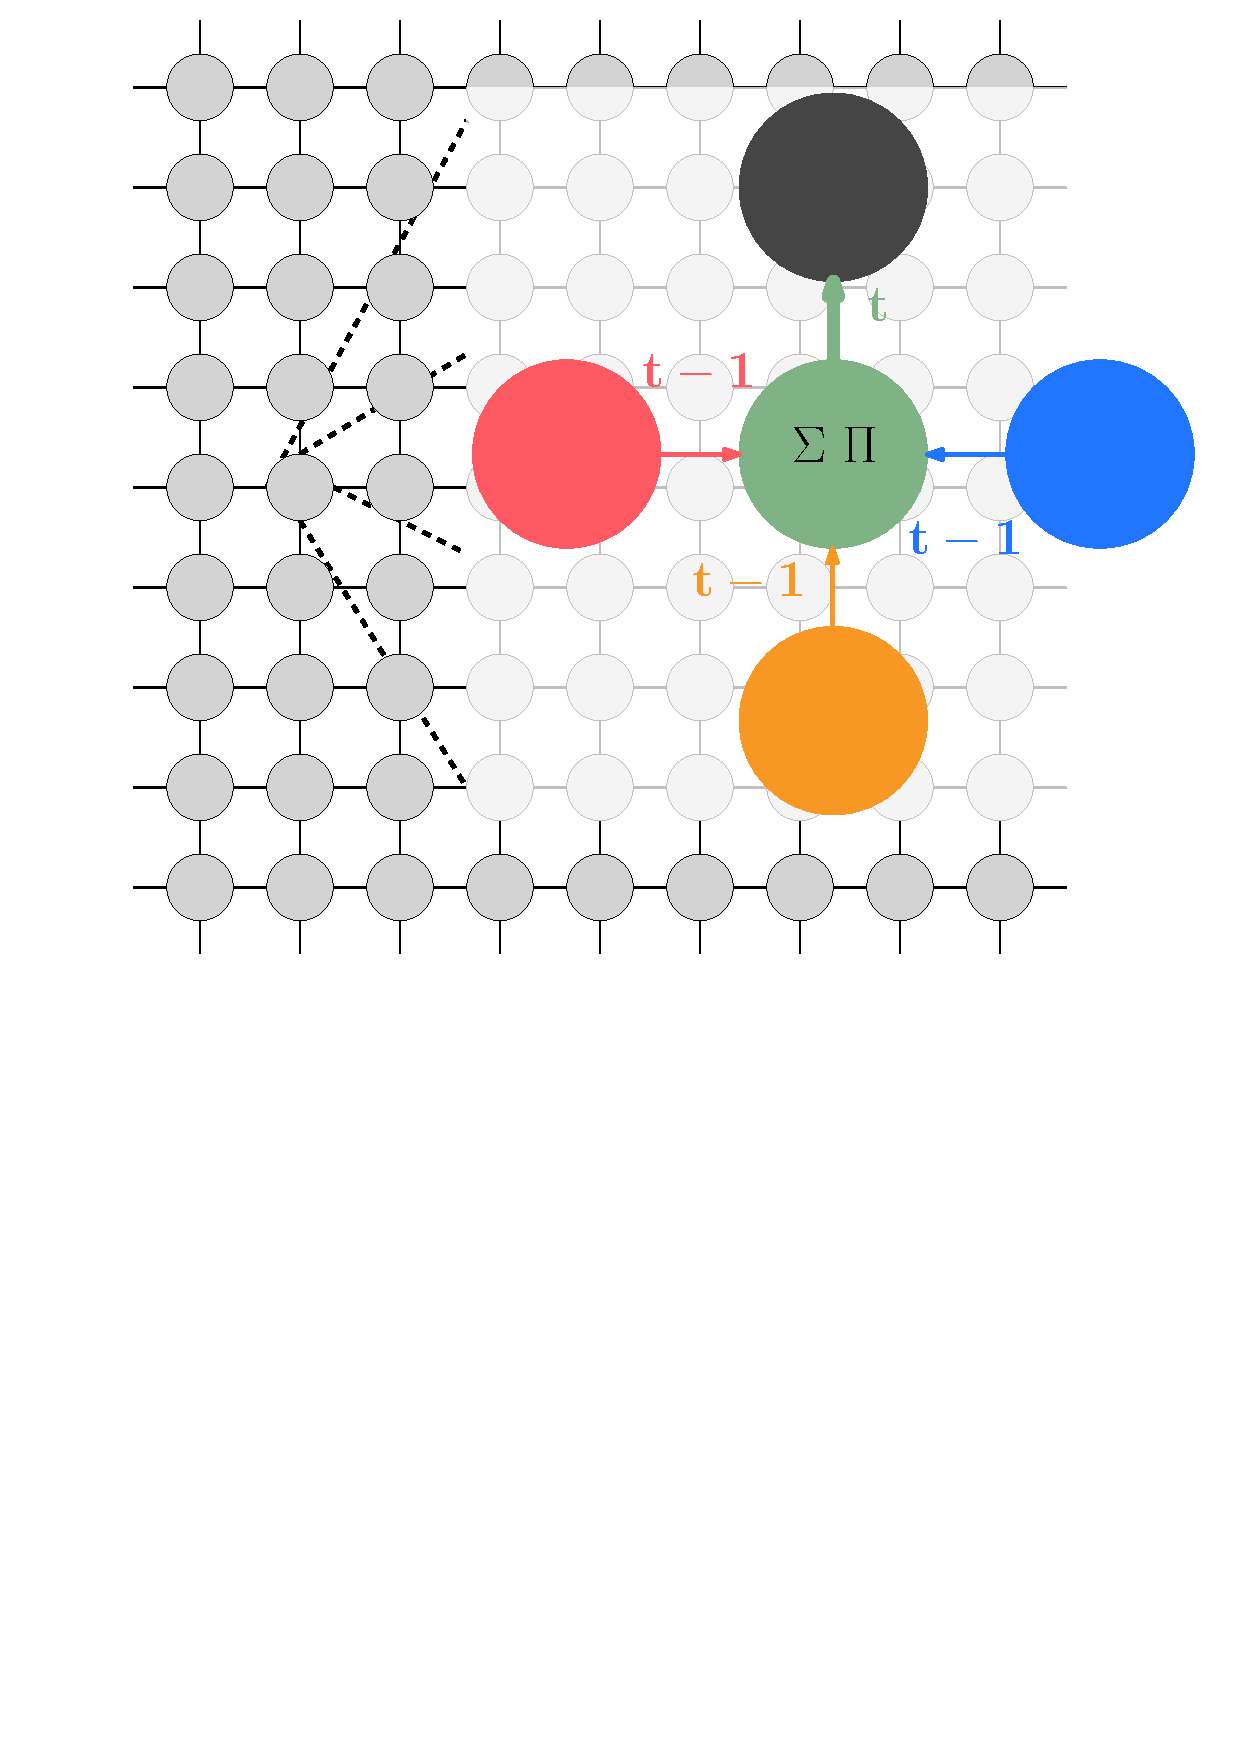
\includegraphics[width=1.0\textwidth]{chapters/litreview/images/bp_diagram_recoloured.pdf}
    \caption[Pictorial representation of the concept behind \glsxtrlong{lbp} for \gls{sm}]{Pictorial representation of the concept behind Loopy Belief Propagation for Stereo Matching. The symbols in the central cell refer to sum-product Belief Propagation, one of the earliest and mostly widely discussed forms of Belief Propagation. Each cell sends a new message to its neighbouring cells at each iteration after in turn having received and processed new messages from the neighbours in the previous iteration. The outgoing message to a given neighbour is computed from the information received from the other neighbours previously, represented here by the three thin and one fat arrow.  Image from \cite{lbpmpsmpic}.}
    \label{fig:bpdiagram}
\end{figure}

Yang \textit{et al.} \cite{Yang2006a} built upon \fxerror*{Explain hierarchical BP}{hierarchical \gls{bp}}, adding in extra steps before and after the \gls{bp} process.  They combine information derived from using the mean shift algorithm \cite{Comaniciu2002}; a colour-weighted correlation method based on Yoon \& Kweon's \cite{Yoon2006} applied to both the left and right images; a left-right consistency check to detect occluded pixels; a plane-fitting process based on Tao \& Sawhney's \cite{Tao2000}; as well as \gls{bp} itself.  While combining these various techniques leads to a highly-accurate disparity map,\footnote{This algorithm achieved the top ranking on Middlebury when it was first introduced.} this approach is \emph{extremely} slow.

Typical \gls{bp} uses the four-connected neighbourhood to define the neighbours of each given node in the grid.  This means that each node passes messages to and from it's immediate neighbours up, down and to the left and right of it in the grid.  Other neighbourhood arrangements are possible though, depending on the underlying model one wants to use.  For example, Tan \textit{et al.} \cite{Tan2017} describe an approach to \gls{bp} where every pixel is considered to be a neighbour of every other pixel.  Messages are weighted according to the distance across the grid between the neighbours, with nearer neighbours having a greater impact upon a pixel's final beliefs.  The major advantage of this approach is that it almost eliminates the need for repeated iterations of message passing.

Ha and Jeong \cite{Ha2016} suggested a different approach for scheduling the messages.  Instead of each pixel repeatedly exchanging messages with its neighbours until a reasonable amount of the grid has been spanned, they start in one of the corners in the image, and sequentially pass messages along two directions until reaching the other corner, repeating this process once for each corner.  The great advantage of this is that in principle one only needs to perform message exchanges in each direction once.  Their implementation still required roughly \SI{3.5}{\second} to complete, however, without returning a significantly more accurate disparity map.\footnote{The authors claimed that their method was \numrange{300}{600} times faster than `standard` \gls{bp}, but they did not specify their stopping condition.  Based on their reported results it appears that they used well over 300 iterations on an image with their standard comparison -- many more than would be reasonable for image sizes likely to be targeted for real-time \gls{sm}.}

Balossino \textit{et al.} \cite{Balossino2007} suggested an alternative formulation to the traditional grid of \gls{lbp}.  Instead, they built a forest of trees, each of which was rooted at the given pixel under consideration, and which has a handful of neighbouring pixels as children.  The attraction of this approach is that it restores the properties of optimality and convergence described in \cite{Pearl1982} for one round of messages up and down each tree.  This advantage is tempered, however, by the necessity of combining results from different trees.  The final accuracy appeared to be worse than with \cite{Felzenszwalb2006}, and there was no reporting of the running time, though it seems unlikely that this approach was fast.

It should be noted that \gls{bp} is \emph{not} regarded as the current top-performing \gls{sm} algorithm.  Tippets \textit{et al.} found c. 2012 that, of algorithms implemented on the CPU, SADL from \cite{VanDerMark2006} was the fastest accurate-enough method, and ADCensus from \cite{Mei2011} was the most accurate, and in fact was described as ``Pareto-optimal'' by Tippets \textit{et al.}  \fxnote{Move this paragraph?}  In terms of \gls{gpu} implementations, the algorithm from \cite{Zhao2011} was the fastest by far (though it only properly worked when observing scenes with motion).  The authors do not state an overall most-accurate \gls{gpu}-based algorithm, but based on Fig. 7 in \cite{Tippetts2016}, it appears that the \gls{gpu} implementation of the ADCensus algorithm from \cite{Mei2011} was again the best.\footnote{Other, faster, algorithms were also discussed, but those required specialist hardware such as \glspl{fpga} or \glspl{dsp}.}  \Gls{bp} \emph{is} amenable to parallelisation (unlike its traditional rival, Graph Cuts \cite{Tappen2003}) and \gls{gpu} implementations, but the main point of interest for it in this work is the fact that it is explicitly built around the concept of independent processing elements exchanging messages.

\begin{anfxwarning}{Top algos on Middlebury}
    Thinking about it, I probably should investigate the current top-performing algorithms on Middlebury, at least the ones which have accompanying publications.
\end{anfxwarning}

\subsubsection{Real-time/resource-constrained \glsentrylong{bp}}
One of the major drawbacks of \gls{bp} as compared to a number of other approaches to \gls{sm} is that a simple naïve implementation is both quite slow, and very memory-intensive.  Slow because of the requirement to perform many iterations, and memory-intensive because \emph{at least} one copy of the data costs and the message estimates for each neighbour must be stored in memory, with the result that a number of values on the order of at least \(O(5XYD)\) are kept in memory, where X and Y are the width and height of the stereo images, and D is the size of the disparity range.

Seeking to derive the comparative benefits of a global stereo algorithm without compromising resource and time requirements too much, there have been a number of attempts at a real-time \gls{bp} algorithm \cite{Liang2011,Perez2010}.

Felzenszwalb \& Huttenlocher \cite{Felzenszwalb2006} made three significant improvements:  i) They demonstrated a way to reduce the complexity of the message update process from \(O(|D|^2)\) to \(O(|D|)\) (where \(|D|\) is the total number of potential disparity labels).  ii) They showed that, because each pixel relies entirely upon the messages received from its neighbours at the previous iteration, only half of the pixels in fact need to be updated in a given iteration, without affecting the final results.  This both halves the number of message computations required for each iteration, but moreover means that only a single copy of the messages need be kept while ensuring that messages computed earlier in an iteration have no impact upon messages computed later.  iii)  They introduced a hierarchical approach, where the first iterations were performed over a much smaller grid, representing an amalgamation of the actual grid, but later iterations would operate over larger and larger grids until reaching the full size.  This had the benefit of propagating information across the grid in a much faster fashion, with relatively little loss in accuracy.  Almost every claimed real-time \gls{bp} algorithm since uses the hierarchical approach.

Notably, Tippetts \textit{et al.} characterised the final algorithm implemented in \cite{Felzenszwalb2006} as Pareto-optimal against almost all other CPU-based \gls{sm} algorithms that they examined, suggesting that there were only five others which provided either better accuracy \emph{or} faster runtimes.  Of course, in the meantime there likely have been improvements in both metrics by newer algorithms.

Yang \textit{et al.} \cite{Yang2006} claimed that they had devised a new approach that would provide a 45x speedup, and boasted that their system could achieve a frame rate of 16 \gls{fps} on a 320 x 240 image with 16 disparity levels.  This claim was largely based, however, in the fact that they used a \gls{gpu} to implement it -- but later stated that they had not yet implemented their method on a \gls{gpu}.  Furthermore, they did not present anything conceptual that had not already been described in \cite{Felzenszwalb2006}. %by Felzenszwalb \& Huttenlocher.

Yu \textit{et al.} \cite{Yu2007} presented a proposed approach for compressing the messages, thus reducing total memory occupied, but it has not proven popular.  This may be because it is not amenable to parallelisation, thus significantly reducing its practicality \cite{Yang2010}.

Yang, Wang \& Ahuja \cite{Yang2010} proposed an approach which they claim needs only constant memory space, regardless of the number of disparities involved, while still returning results that are almost as accurate.  For example, they claim that for an image with 800 x 600 pixels and 300 disparity levels, their algorithm requires only around \SI{9}{\mebi\byte} of memory --- though it is not clear though whether they include storing the computed data costs in that amount or not.  The main element of their approach is that as they move from the coarser levels of the hierarchy, they proportionally reduce the number of disparity labels considered at each level, keeping the total memory required constant.  %This leads to an issue in that, should the true disparity not be selected for inclusion at a reduction, that pixel will never see the correct disparity label assigned to it.  To work around this, they 

Gupta \& Cho \cite{Gupta2012} used 3x3 tiles in their hierarchical method, rather than the usual 2x2.  This meant that their process was somewhat faster overall, and means that at the more coarse levels they need less memory.  The other main differences between their method and previous ones are that they use an `alternative schedule method' borrowed from \cite{Tappen2003}; and they use a different disparity refinement operation as final step.  The results, in terms of accuracy and speed, do not appear to be any better than earlier papers, though.

Xiang \textit{et al.} \cite{Xiang2012} also boasted of a new technique that enabled faster speeds, but again their implementation largely merely borrowed concepts from \cite{Felzenszwalb2006} and used a \gls{gpu}.  They did improve accuracy results, however, by incorporating Yoon \& Kweon's \cite{Yoon2005} adaptive support-weight approach as a post-processing step, with minimal extra computational requirements.

Tan \textit{et al.} \cite{Tan2017} claim that their fully-connected \gls{bp} method is highly-amenable to parallelisation, suggesting it could be implemented to run in real-time, but they do not appear to have done so themselves.

% \cite{Gong2015,Gong2013a}

% \subsection{Message Passing \glsentrytext{sm} -- other?}
% Look at, \eg{}:
% Tan, X. et al. (2017) ‘Efficient Message Passing Methods With Fully Connected Models for Early Vision’, IEEE Transactions on Image Processing, 26(12), pp. 5994–6005. doi: 10.1109/TIP.2017.2750406.
% Ružic, T., Pižurica, A. and Philips, W. (2011) ‘Neighbourhood-consensus message passing and its potentials in image processing applications’, in Astola, J. T. and Egiazarian, K. O. (eds) Image Processing: Algorithms and Systems IX. San Francisco: Society of Photo-Optical Instrumentation Engineers, p. 78700Z. doi: 10.1117/12.872464.
% Ružić, T., Pižurica, A. and Philips, W. (2012) ‘Neighborhood-consensus message passing as a framework for generalized iterated conditional expectations’, Pattern Recognition Letters, 33(3), pp. 309–318. doi: 10.1016/j.patrec.2011.10.014.
% Szeliski, R. et al. (2008) ‘A Comparative Study of Energy Minimization Methods for Markov Random Fields with Smoothness-Based Priors’, IEEE Transactions on Pattern Analysis and Machine Intelligence, 30(6), pp. 1068–1080. doi: 10.1109/TPAMI.2007.70844.
% Thomas, D. et al. (2019) ‘Revisiting Depth Image Fusion with Variational Message Passing’, in 2019 International Conference on 3D Vision (3DV). IEEE, pp. 328–337. doi: 10.1109/3DV.2019.00044.

